% Please provide a full mailing address here.
% \title{}
% \author{Warren}
% \author{}
% \author{}
% \author{Lemon}

This chapter is a reprint of published paper: \\
Warren$^{\dagger}$, Lemon$^{\dagger}$, \textit{Journal Name} \textbf{Year} \\ %In this chapter, we...
DOI: XXX

$^{\dagger}$These authors contributed equally to the reproduced part in this thesis.

% This chapter is adapted from the preprint version of ..., submitted to Some Journal. In this chapter, we... 

\section*{abstract}
\lipsum[1]



\section{Introduction}
\lipsum[2]

Example of a Figure reference Fig. \ref{fig:ch1-patent}. 
Example of a Three-part table reference Fig. \ref{tbl:ch1-table}. 
Example of a SI Figure reference Fig.~\ref{fig:ch1si-patent}.
Example of a SI table reference Fig. \ref{tbl:ch1si-table}.


\begin{figure}
\centering
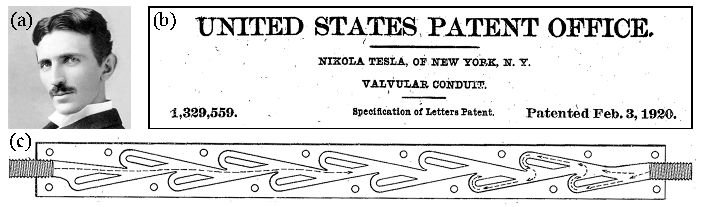
\includegraphics[width=16.5cm]{figures/ch_chapter1/fig1.pdf}\vspace{-0.2cm}
\caption{(a) The genius Nikola Tesla (b) His patent (c) Tesla's channel }
\label{fig:ch1-patent}
\end{figure}

\begin{table}
\centering
\caption{Data sheet}
\label{tbl:ch1-table}
\begin{threeparttable}
\begin{tabular}{lcccccc}
\toprule
{} &   \specialcell{Column 1}  & \specialcell{Column 2} & \specialcell{Column 3} & \specialcell{Column 4} \\
\midrule
A &  B  & C &  D & E\\
A  &  B & C & D & E \\
A  &  B & C & D & E \\
A  &  B & C & D & E \\
A  &  B & C & D & E \\
A  &  B & C & D & E \\
A  &  B & C & D & E \\
\bottomrule
\end{tabular}
\begin{tablenotes}
\small
\item Notes Notes Notes Notes Notes Notes Notes Notes Notes
\end{tablenotes}
\end{threeparttable}
\end{table}